\chapter{Overlapping, heterogeneous age groups: atrial fibrillation}
\label{applications-age_groups}

Atrial fibrillation research has no standard set of age groups for
study.  Therefore the meta-analysis of data from systematic review on
the descriptive epidemiology parameters of atrial fibrillation
provides an excellent example of overlapping and heterogeneous age
groups.

Atrial fibrillation is the most common type of cardiac arrhythmia.
Chaotic and irregular heart rhythms originating in the atria cause
poor blood flow to the body.  Atrial fibrillation episodes may be
occasional, only lasting a few minutes or hours, or chronic if the
heart rhythm is always abnormal.  Symptoms include heart palpitations,
lack of energy, dizziness, shortness of breath and chest discomfort,
although some cases of atrial fibrillation are symptomless.  Atrial
fibrillation may occur at any age with increasing risk for older ages.
It is uncommon in children. \cite{rich_epidemiology_2009,
  rho_asymptomatic_2005, fuster_acc/aha/esc_2006, radford_atrial_1977}

For analysis, atrial fibrillation in Western Europe has 229 data
points.  As seen from Figure \ref{fig:app-af data}, atrial
fibrillation has heterogeneous and overlapping age groups.  Without
access to the microdata needed to recreate homogeneous age groups, combining all of this data must rely on age group modeling, as described in Chapter~\ref{chap:age_group_model}.

    \begin{figure}[h]
        \begin{center}
            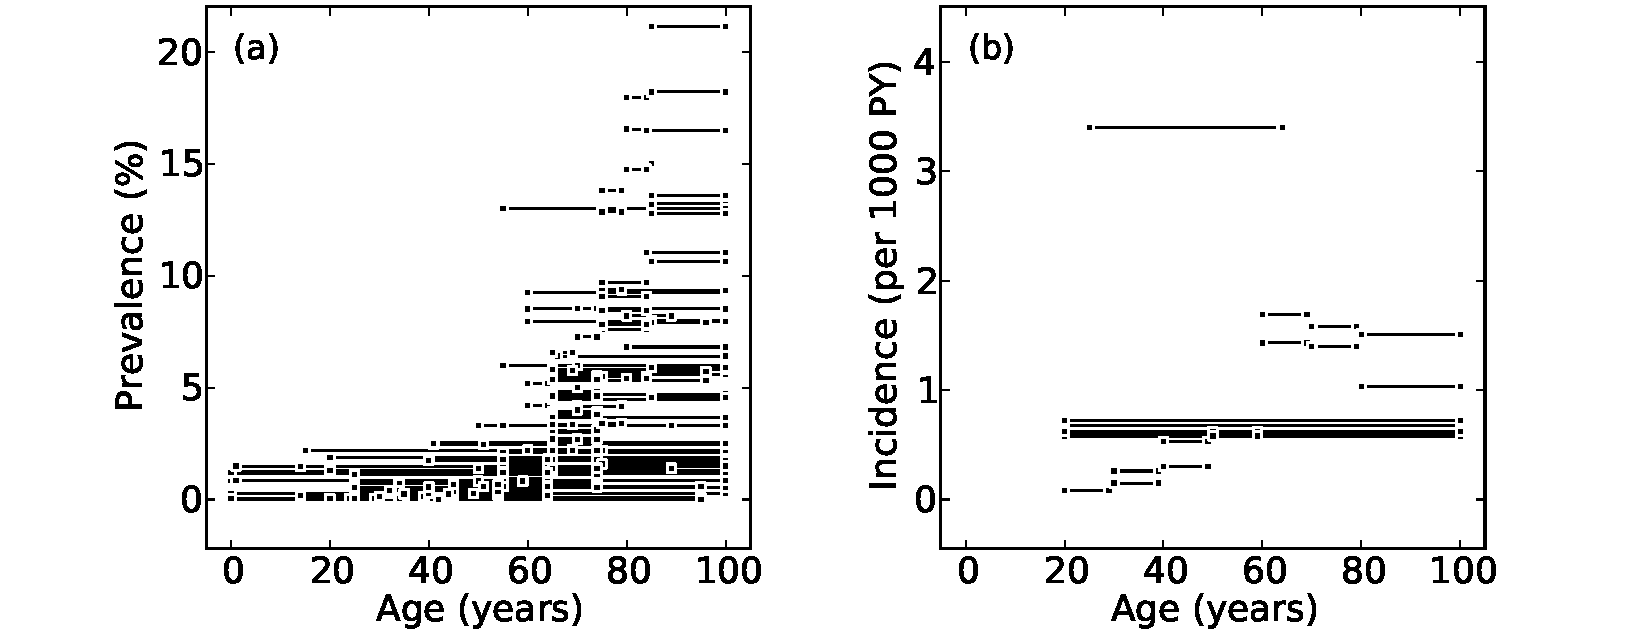
\includegraphics[width=\textwidth]{af-data.pdf}
            \caption{Data for Western Europe males with atrial
              fibrillation is an excellent example of heterogeneous
              and overlapping age groups.}
            \label{fig:app-af data}
        \end{center}
    \end{figure}

As discussed in Chapter \ref{theory-age_group_model-overlapping_data},
the simplest approach to modeling heterogeneous age groups is to apply
each age-specific rate measurement to the midpoint of the age interval.
Another solution to the heterogeneous age groups is to use age-standardizing.
Age-standardizing adds age-weights to the age-specific rate according
to population structure.  The age-standardizing model uses a common
age pattern for all studies so that the age-weights are the same for
all age groups, as discussed in more detail in Chapter
\ref{theory-age_group_model-overlapping_data}.

As the prevalence estimates in Figure \ref{fig:app-af srt p} show, model
choice matters.  While the midpoint and age-standardizing models produce
similar estimates for younger ages, the estimates for the oldest age groups
differ in magnitude and trend.

    \begin{figure}[h]
        \begin{center}
            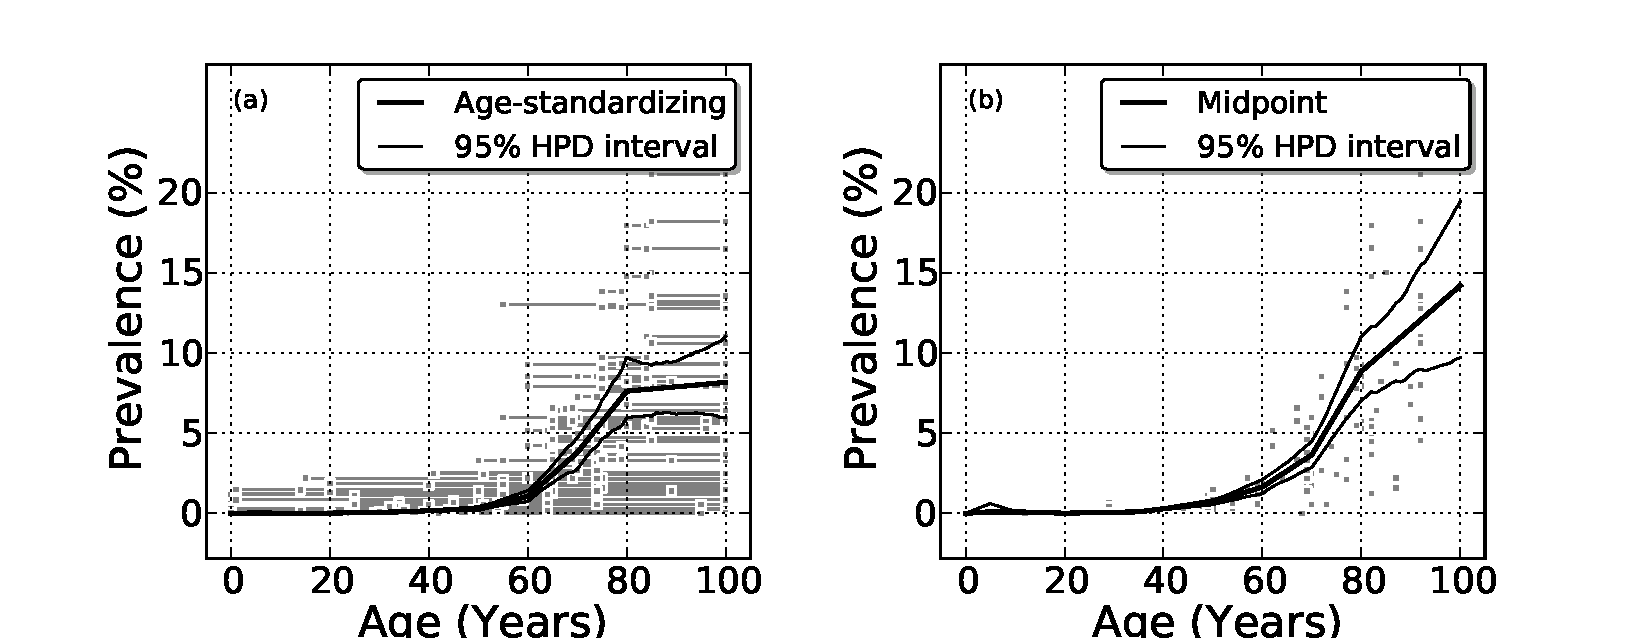
\includegraphics[width=\textwidth]{af-mp_v_hetero_srt_p.pdf}
            \caption{Comparison of prevalence estimates for Western European
              males with atrial fibrillation in 1990 using an age-standardizing
              or midpoint spline model.  Panel (a) shows the data and 
              estimates for the age-standardizing model and panel (b)
              ddata used the midpoint model.}
            \label{fig:app-af srt p}
        \end{center}
    \end{figure}

Without additional information, one cannot say which model is correct.
Further investigation with incidence does not provide much insight.  Like
the prevalence estimates, Figure \ref{fig:app-af srt i} shows that the
incidence estimates are similar in younger ages, but are markedly different
in older ages.  The age-standardizing model does produce estimates with a
smoother age pattern.

    \begin{figure}[h]
        \begin{center}
            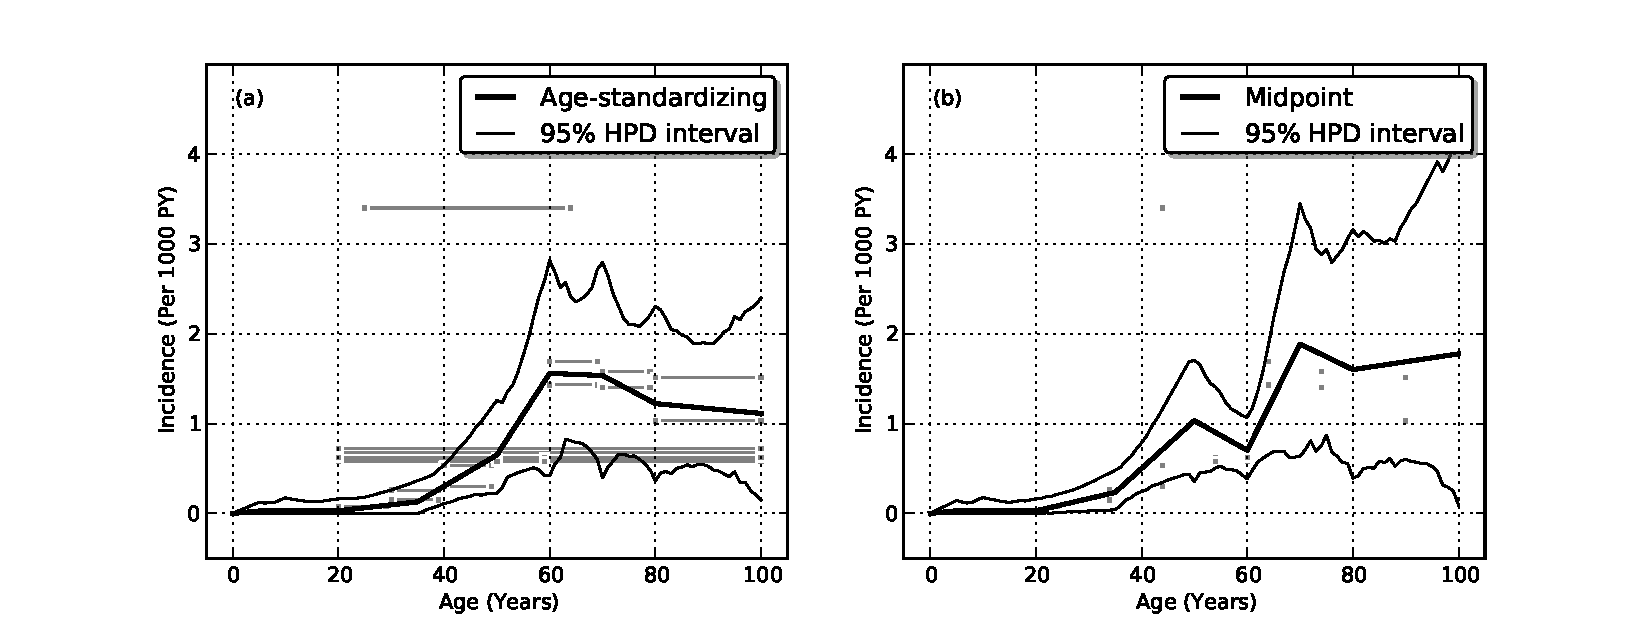
\includegraphics[width=\textwidth]{af-mp_v_hetero_srt_i.pdf}
            \caption{Comparison of incidence estimates for Western European
              males with atrial fibrillation in 1990 using an age-standardizing
              or midpoint spline model.}
            \label{fig:app-af srt i}
        \end{center}
    \end{figure}
    
Using of all available data in a compartmental model, including the 
limited available data on excess mortality, with-condition mortality 
and cause-specific mortality, could inform the model choice.  
A compartmental model simultaneously estimates all parameters to 
maintain internal consistency.  Compartmental models are discussed 
in more discussed in more detail in Chapters \ref{sys-dynamics}.  
Figure \ref{fig:app-af age-stand} shows prevalence and incidence estimates 
from the age-standardizing compartmental.

The compartmental model estimates from Figure \ref{fig:app-af age-stand} 
are very different from the spline model estimates, especially for incidence.  
Unlike the spline models, the compartmental model estimates for 
incidence do not go through the data.  This is because the compartmental model 
requires internal consistency, i.e. for every prevalent case there must be 
a matching incident event.  The compartmental model shows that these levels 
of prevalence cannot be achieved with the levels of incidence the data show.

    \begin{figure}[h]
        \begin{center}
            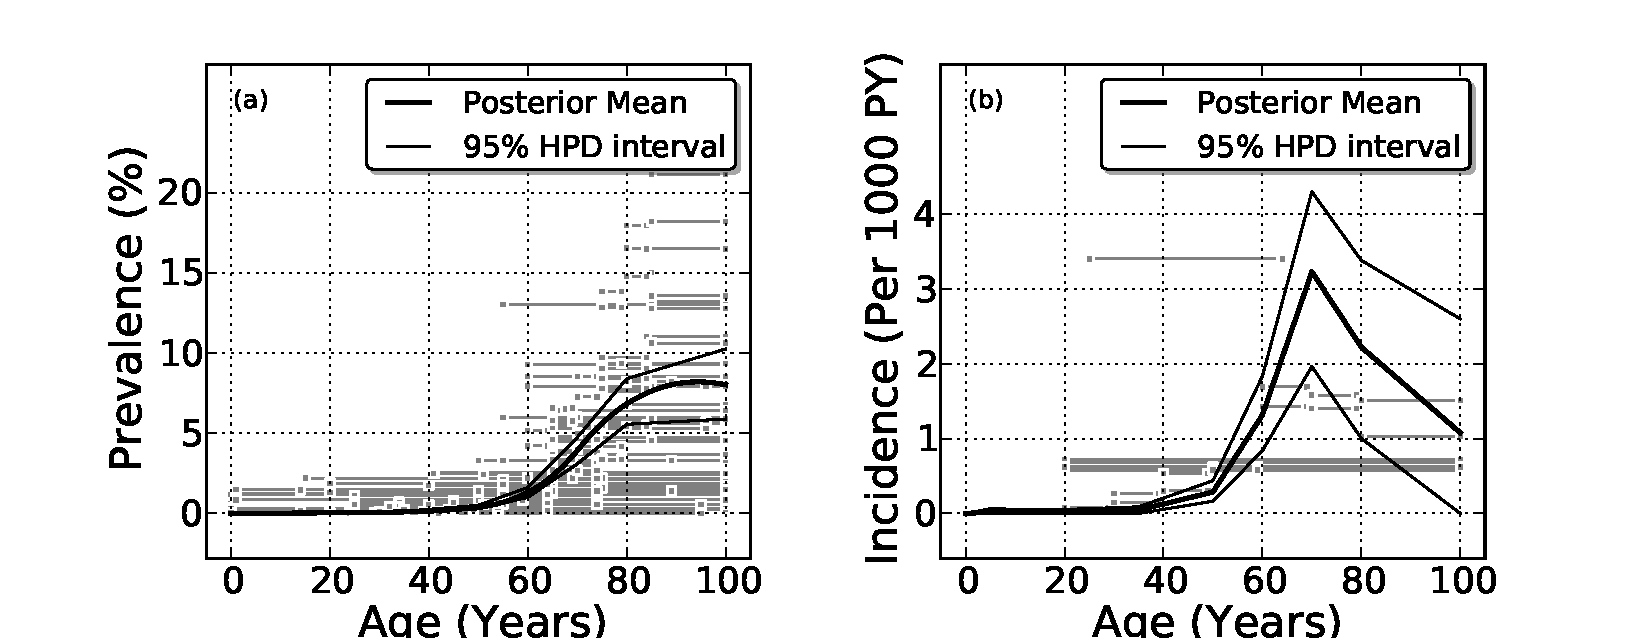
\includegraphics[width=\textwidth]{af-best_model.pdf}
            \caption{Estimates of prevalence (panel (a)) and incidence (panel (b))
              of atrial fibrillation in males in Western European in 1990 using
              an age-standardizing compartmental model.}
            \label{fig:app-af age-stand}
        \end{center}
    \end{figure}

Figure \ref{fig:app-af compare} compares the age-standardizing compartmental 
model to the midpoint compartmental model.  Like the spline models, 
the prevalence estimates only differ in the oldest ages.  However, the 
incidence of the two models is very different.  The age-standardizing model 
has an earlier age of onset and decline than the midpoint model.

    \begin{figure}[h]
        \begin{center}
            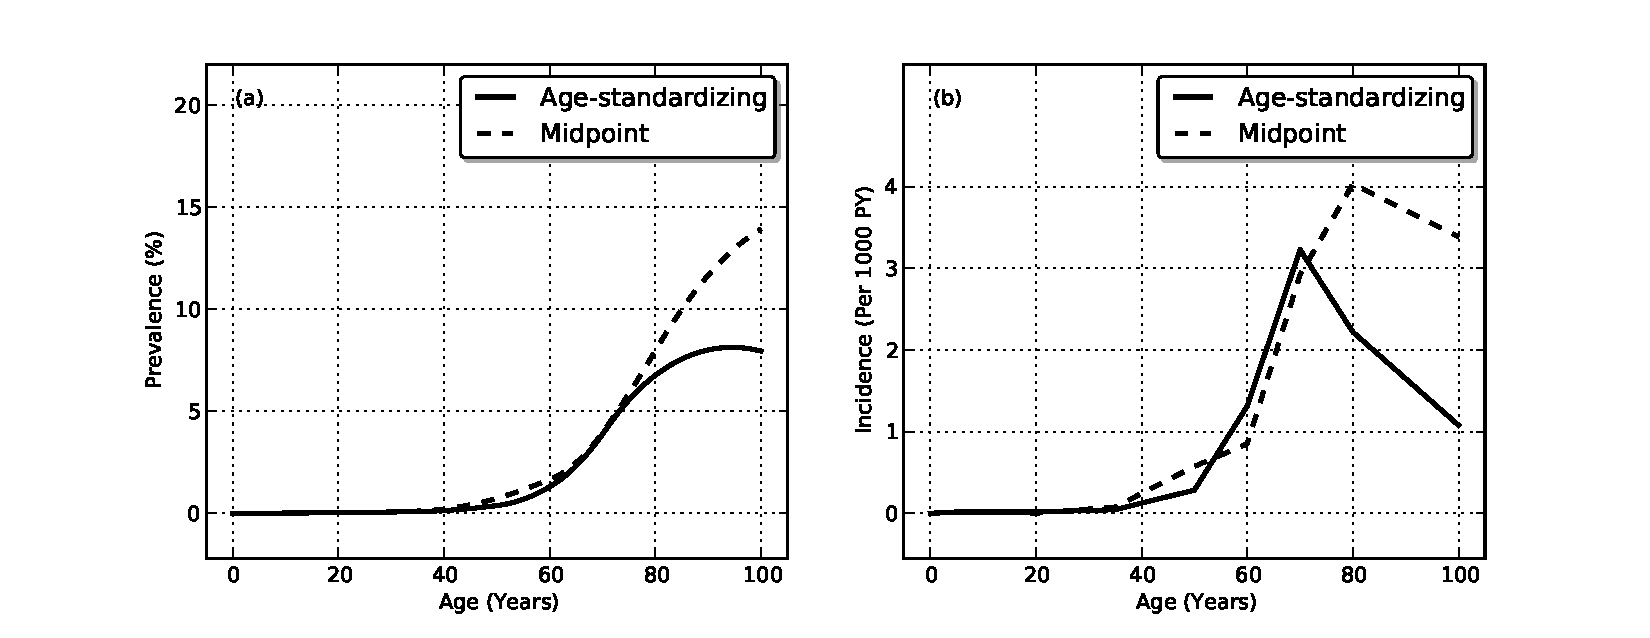
\includegraphics[width=\textwidth]{af-mp_v_hetero.pdf}
            \caption{A comparison of the estimated prevalence (panel (a)) and incidence (panel
              (a)) in Western European males with atrial fibrillation in 1990 using
              an age-standardizing and midpoint compartmental models.}
            \label{fig:app-af compare}
        \end{center}
    \end{figure}
